\documentclass{article}

\oddsidemargin -6mm
\evensidemargin -10mm
\textwidth 160mm
\textheight 200mm
\renewcommand\baselinestretch{1.0}

\pagestyle{plain}
\pagenumbering{arabic}

\usepackage{amsfonts}
\usepackage{graphicx}

\title{Assignment 4, Part 1, Specification}
\author{Ethan Vince-Budan}

\begin{document}

\maketitle

This Module Interface Specification document contains modules, types and methods for implementing the game \textit{2048}. $2048$ is a game about merging tiles of similar values, and trying to reach the highest possible score before getting stuck. The player can do this by shuffling the tiles on the board in one of four directions: up, down, left and right. On each turn, the player decides which way they would like to move, and every tile on the board attempts to move as far as possible in that direction. If two tiles of similar value collide during their move, they can merge into a tile of higher value. This rewards the player with some points. At the end of each turn, a new low-value tile is placed somewhere random on the board. The game is over once no more tiles can be moved, and no more merges can be made. The game can be launched and played by using the command \textbf{make demo} in a terminal.

Throughout this document, a \textit{row} is a horizontal line of tile from end to end of the board. Similary, a \textit{column} is a vertical line. A cell or tile is an individual piece on the board, which must occupy one of the 16 spaces on the board. In this implementation, an empty cell is a cell with a value of zero.

\section{Overview of the Design}
	\subsection{Description of Classes}
		This implementation uses a model-view-controller (MVC) design pattern, for controlling the graphical user interface and updaing the board during each turn. The view module, labeled as $GUI$, provides the graphical interface to the user, as well as a means for them to input instructions into the game. Display of the board itself is handled by a seperate class called a BoardDisplay, which holds all the specific information such as colors and coordinates which are used to display the tiles. Input from the user is captured by the $GUI$ object and sent to the controller portion of MVC.

		The Controller handles the input given by the user, decoding the user's intentions from their input and sending commands to the model portion of the MVC pattern. The Controller also tells the GUI to update whenever a move has been completed, so the user can have the correct information displayed on the screen. The controller acts as the bridge between the GUI and the model, which is where all the actual state information for the game is stored.

		The Model handles the manipulation of data, and stores anything state related about the game. To store the actual board data, a seperate class BoardStorage stores the board information, while the manipulation of this board data is done throught the Movement class, which holds the algorithms necessary to modify the board data during a turn. A Score class is invoked by the Movement class to update the scores stored in the Board class, and could potentially hold many different types of scoring schemes for different modes of gameplay.

\newpage

\section{Module Interface Specification}

\section*{Directions Module}

	\subsection*{Module}
		Direction

	\subsection*{Uses}
		None

	\subsection*{Syntax}

		\subsubsection*{Exported Constants}
			None

		\subsubsection*{Exported Types}
			Directions = \{\\
				UP,\\
				DOWN,\\
				LEFT,\\
				RIGHT\\
			\}

		\subsubsection*{Exported Access Programs}
			None

	\subsection*{Semantics}

		\subsubsection*{State Variables}
			None

		\subsubsection*{State Invariant}
			None

		\subsubsection*{Assumptions}
			None

		\subsubsection*{Considerations}
			This class should be implemented as an enumerated type.

\newpage

\section*{Board Storage Module}

	\subsection*{Template Module}
		BoardStorage

	\subsection*{Uses}
		None

	\subsection*{Syntax}

		\subsubsection*{Exported Constants}
			None

		\subsubsection*{Exported Types}
			BoardStorage = ?

		\subsubsection*{Exported Access Programs}
			\begin{tabular}{|l|l|l|p{5cm}|}
				\hline
				\textbf{Routine Name} & \textbf{In} & \textbf{Out} & \textbf{Exceptions} \\
				\hline
				new BoardStorage & $\mathbb{N}, \mathbb{N}$ & BoardStorage & IllegalArgumentException\\
				\hline
				setRow & $\mathbb{N}$, seq of $\mathbb{Z}$ & & IllegalArgumentException\\
				\hline
				setCol & $\mathbb{N}$, seq of $\mathbb{Z}$ & & IllegalArgumentException\\
				\hline
				getWidth & & $\mathbb{N}$ & \\
				\hline
				getHeight & & $\mathbb{N}$ & \\
				\hline
				getBoard & & seq of (seq of $\mathbb{Z}$) & \\
				\hline
				isFull & & $\mathbb{B}$ & \\
				\hline
				addRandomTiles & $\mathbb{N}$ & & ArrayStoreException \\
				\hline
				getTileAt & $\mathbb{N}, \mathbb{N}$ & & \\
				\hline
			\end{tabular}

	\subsection*{Semantics}

		\subsubsection*{State Variables}
			\textit{contents} : seq of (seq of $\mathbb{Z}$)\\
			\textit{width} : $\mathbb{N}$\\
			\textit{height} : $\mathbb{N}$

		\subsubsection*{State Invariant}
			$|contents| = height \wedge |contents[0]| = width$

		\subsubsection*{Assumptions}
			None

		\subsubsection*{Access Routine Semantics}
			\noindent new BoardStorage(\textit{x}, \textit{y}):
			\begin{itemize}
				\item transition: \textit{width}, \textit{height}, \textit{contents} := 
					$\mathit{x}, \mathit{y}, \langle \forall j : \mathbb{N} | j \in [0..\textit{y}-1] : \langle \forall i : \mathbb{N} | i \in [0..\textit{x}-1] : 0 \rangle \rangle$ \# Initialize a 2D-array of zeros.
				\item output: \textit{out} := \textit{self}
				\item exception: exc := $((\mathit{x} \le 1 \vee \mathit{y} \le 1) \Rightarrow \textrm{IllegalArgumentException})$
			\end{itemize}

			\noindent setRow(\textit{n}, \textit{row}):
			\begin{itemize}
				\item transition: \textit{contents}[n] := $\mathit{row}$ \# Replace row n with \textit{row}.
				\item exception: exc := $(n \notin [0..height-1] \vee |row| \neq width) \Rightarrow \textrm{IllegalArgumentException}$
			\end{itemize}

			\noindent setCol(\textit{n}, \textit{col}):
			\begin{itemize}
				\item transition: \textit{contents} := $\forall y : \mathbb{N} | (y \in [0..\textit{height}-1] \Rightarrow contents[y][n] = \mathit{col}[y])$\\
					\# Replace every value in column n with corresponding value from \textit{col}.
				\item exception: exc := $(n \notin [0..width-1] \vee |col| \neq height) \Rightarrow \textrm{IllegalArgumentException}$
			\end{itemize}

			\noindent getWidth():
			\begin{itemize}
				\item output: \textit{out} := \textit{width}
				\item exception: None
			\end{itemize}

			\noindent getHeight():
			\begin{itemize}
				\item output: \textit{out} := \textit{height}
				\item exception: None
			\end{itemize}

			\noindent getBoard():
			\begin{itemize}
				\item output: \textit{out} := \textit{contents}
				\item exception: None
			\end{itemize}

			\noindent isFull():
			\begin{itemize}
				\item output: \textit{out} := $\wedge\{y : \mathbb{N} | y \in [0..\textit{height}-1] : \{ x : \mathbb{N} | x \in [0..\textit{width}-1] : \textit{contents}[y][x] \neq 0\}\}$ \# Returns \textit{True} if all cells are nonzero
				\item exception: None
			\end{itemize}

			\noindent addRandomTiles(\textit{n}):
			\begin{itemize}
				\item transition: $\forall i : \mathbb{N} | i \in [0..n] : contents[Random.next()*height][Random.next()*width] = 0 \Rightarrow contents[Random.next()*height][Random.next()*width] = (Random.next() < 0.9 \Rightarrow 2 | True \Rightarrow 4)$ \# Add n tiles to the board in random empty positions, with a 10\% chance of being a 4 and a 90\% chance of being a 2.
				\item exception: $exc := (isFull() \Rightarrow \textrm{ArrayStoreException})$
			\end{itemize}

			\noindent getTileAt(\textit{x}, \textit{y})
			\begin{itemize}
				\item output: $out := ((x \in [0..width-1] \wedge y \in [0..height-1]) \Rightarrow contents[y][x]) | (True \Rightarrow -1)$ \# Return value of tile at position, if position out of bounds return -1
				\item exception: None
			\end{itemize}

\newpage

\section*{Movement Algorithms Module}
	
	\subsection*{Module}
		Movement

	\subsection*{Uses}
		Direction, Score

	\subsection*{Syntax}

		\subsubsection*{Exported Constants}
			None

		\subsubsection*{Exported Types}
			None

		\subsubsection*{Exported Access Programs}
			\begin{tabular}{|l|l|l|p{5cm}|}
				\hline
				\textbf{Routine Name} & \textbf{In} & \textbf{Out} & \textbf{Exceptions} \\
				\hline
				shift & Direction, seq of $\mathbb{Z}$ & seq of $\mathbb{Z}$ & \\
				\hline
				moveMade & & $\mathbb{B}$ & \\
				\hline
				clearMoveMade & & & \\
				\hline
			\end{tabular}

	\subsection*{Semantics}

		\subsubsection*{State Variables}
			\textit{moveMade} : $\mathbb{B}$

		\subsubsection*{State Invariant}
			None

		\subsubsection*{Assumptions}
			the \textit{moveMade} state variable should be initialized to \textit{False}.

		\subsubsection*{Access Routine Semantics}
			\noindent moveMade():
			\begin{itemize}
				\item output: $out := moveMade$
				\item exception: None
			\end{itemize}

			\noindent clearMoveMade():
			\begin{itemize}
				\item transition: $moveMade := false$
				\item exception: None
			\end{itemize}

			\noindent shift(\textit{dir}, \textit{seq}):
			\begin{itemize}
				\item output: $out := (dir = Direction.UP \vee dir = Direction.LEFT) \Rightarrow shiftLeft(seq) | (dir = Direction.DOWN \vee dir = Direction.RIGHT) \Rightarrow shiftRight(seq)$
			\end{itemize}

	\subsection*{Local Functions}
		\noindent shiftLeft: seq of $\mathbb{Z} \rightarrow$ seq of $\mathbb{Z}$\\
		\noindent shiftLeft(\textit{seq}) $\equiv (\forall i : \mathbb{N} | i \in [0..|seq|-1] : (\forall j : \mathbb{N} | j \in [1..i] : ((seq[i-1] = seq[i] \wedge \neg merged[i-1]) \vee seq[i-1] = 0) \Rightarrow (seq[i-1] := seq[i-1] + seq[i], Score.updateScore(seq[i-1]-seq[i]), seq[i] := 0)))$\\

		\noindent \# For every entry in $seq$, if the entry to the left of it is equal in value or zero, add the cells values together, update the game score using their difference, and erase the original position. Since empty cells have a value of zero, merging a cell with an empty one results in 0 additional score. NOTE: This algorithm should NOT be greedy, that is cells can only merge once. this could be acheived in many ways, but here we are using a sequence of boolean values $merged$.

		\bigskip

		\noindent shiftRight: seq of $\mathbb{Z} \rightarrow$ seq of $\mathbb{Z}$\\
		\noindent shiftRight(\textit{seq}) $\equiv (\forall i : \mathbb{N} | i \in [0..|seq|-1] : (\forall j : \mathbb{N} | j \in [i..1] : ((seq[i+1] = seq[i] \wedge \neg merged[i+1]) \vee seq[i+1] = 0) \Rightarrow (seq[i+1] := seq[i+1] +  seq[i], Score.updateScore(seq[i+1]-seq[i]), seq[i] := 0)))$\\

		\noindent \# This is the same algorithm as above, but cells are merged to the right instead of to the left. Again, this algorithm should not be greedy, and cells should only merge once. Note that shiftRight starts merging from the rightmost element and traverses leftwards, while shiftLeft starts merging from the leftmost and traverses rightwards.



\newpage

\section*{Score Calculation Module}

	\subsection*{Module}
		Score

	\subsection*{Uses}
		Board

	\subsection*{Syntax}

		\subsubsection*{Exported Constants}
			None

		\subsubsection*{Exported Types}
			None

		\subsubsection*{Exported Access Programs}
			\begin{tabular}{|l|l|l|p{5cm}|}
				\hline
				\textbf{Routine Name} & \textbf{In} & \textbf{Out} & \textbf{Exceptions} \\
				\hline
				updateScore & $\mathbb{Z}$ & &  \\
				\hline
			\end{tabular}

	\subsection*{Semantics}

		\subsubsection*{State Variables}
			None

		\subsubsection*{State Invariant}
			None

		\subsubsection*{Assumptions}
			None

		\subsubsection*{Access Routine Semantics}

			\noindent updateScore(\textit{val}):
			\begin{itemize}
				\item transition: Board.\textit{setScore}(\textit{val})
				\item exception: None
			\end{itemize}

\newpage

\section*{Game State Module (Abstract Object)}
	
	\subsection*{Module inherets BoardStorage}
		Board

	\subsection*{Uses}
		BoardStorage, Movement, Direction

	\subsection*{Syntax}

		\subsubsection*{Exported Constants}
			None

		\subsubsection*{Exported Types}
			None

		\subsubsection*{Exported Access Programs}
			\begin{tabular}{|l|l|l|p{5cm}|}
				\hline
				\textbf{Routine Name} & \textbf{In} & \textbf{Out} & \textbf{Exceptions} \\
				\hline
				init & $\mathbb{N}, \mathbb{N}$ & & IllegalArgumentException \\
				\hline
				move & Direction & & \\
				\hline
				getScore & & $\mathbb{Z}$ & \\
				\hline
				getHighScore & & $\mathbb{Z}$ & \\
				\hline
				setScore & $\mathbb{Z}$ & & \\
				\hline
				movesPossible & & $\mathbb{B}$ & \\
				\hline
				getBoard & & seq of (seq of $\mathbb{Z}$) & \\
				\hline
			\end{tabular}

	\subsection*{Semantics}

		\subsubsection*{State Variables}
			\textit{score} : $\mathbb{Z}$\\
			\textit{highScore} : $\mathbb{Z}$\\
			\textit{contents} : BoardStorage

		\subsubsection*{State Invariant}
			None

		\subsubsection*{Assumptions}
			\begin{itemize}
				\item The init access program will be called before any other access program
				\item Any parameters passed to the access programs will be of the correct type.
			\end{itemize}

		\subsubsection*{Access Routine Semantics}
			\noindent init(\textit{x}, \textit{y}):
			\begin{itemize}
				\item transition: \textit{score}, \textit{highScore}, \textit{contents} := $0, 0, \textrm{new BoardStorage(\textit{x}, \textit{y})}$
				\item exception: $((\mathit{x} \le 1 \vee \mathit{y} \le 1) \Rightarrow IllegalArgumentException)$
			\end{itemize}

			\noindent move(\textit{dir}):
			\begin{itemize}
				\item transition: $(dir = Direction.UP \vee dir = Direction.DOWN) \Rightarrow (\forall i : \mathbb{N} | i \in [0..contents.getWidth()-1] : contents.setCol(i, Movement.shift(dir, contents.getCol(i))))\\ | (dir = Direction.LEFT \vee dir = Direction.RIGHT) \Rightarrow (\forall i : \mathbb{N} | i \in [0..contents.getHeight()-1] : contents.setRow(i, Movement.shift(dir, contents.getCol(i))))$\\
				\# If direction is vertical, update every column to be shifted in the given direction. If direction is horizontal, update every row to be shifted in the given direction.
				\item exception: None
			\end{itemize}

			\noindent getScore():
			\begin{itemize}
				\item output: \textit{out} := \textit{score}
				\item exception: None
			\end{itemize}

			\noindent getHighScore():
			\begin{itemize}
				\item output: \textit{out} := \textit{highScore}
				\item exception: None
			\end{itemize}

			\noindent setScore(\textit{s}):
			\begin{itemize}
				\item transition: \textit{score}, \textit{highScore} := $\mathit{s}, (\mathit{s} > \mathit{highScore} \Rightarrow \mathit{s}) | True \Rightarrow \mathit{highScore}$
				\item Exception: none
			\end{itemize}

			\noindent movesPossible():
			\begin{itemize}
				\item output: $out := (\neg contents.isFull()) \Rightarrow True | True \Rightarrow (\forall y : \mathbb{N} | y \in [0..|contents.getBoard()|-1] : (\forall x : \mathbb{N} | y \in [0..|contents.getBoard()[0]|-1] : ((contents.getTileAt(x, y-1) = contents.getTileAt(x,y) \Rightarrow True | (contents.getTileAt(x, y+1) = contents.getTileAt(x,y) \Rightarrow True | (contents.getTileAt(x-1, y) = contents.getTileAt(x,y) \Rightarrow True | (contents.getTileAt(x+1, y) = contents.getTileAt(x,y) \Rightarrow True) | True \Rightarrow False))$\\
				\# If board is not full, immediately return True. If it is full, check to see if any tiles have neighbors of the same value. If this is true, return True. If no tiles have same-valued neighbors, return False.
				\item exception: None
			\end{itemize}

			\noindent getBoard():
			\begin{itemize}
				\item output: \textit{out} := $\{y : \mathbb{N} | y < \mathit{height} : \mathit{contents}.\textrm{getRow(\textit{i})}\}$
				\item exception: None
			\end{itemize}
\newpage		

\section*{Controller Module}

	\subsection*{Template Module inherets KeyListener, ActionListener}
		Controller

	\subsection*{Uses}
		Board, KeyEvent, KeyListener, ActionListener, ActionEvent

	\subsection*{Syntax}

		\subsubsection*{Exported Constants}
			None

		\subsubsection*{Exported Types}
			Controller = ?

		\subsubsection*{Exported Access Programs}
			\begin{tabular}{|l|l|l|p{5cm}|}
				\hline
				\textbf{Routine Name} & \textbf{In} & \textbf{Out} & \textbf{Exceptions} \\
				\hline
				new Controller & & Controller & \\
				\hline
				keyPressed & KeyEvent & & \\
				\hline
				isGameOver & & & \\
				\hline
				actionPerformed & ActionEvent & & \\
				\hline
			\end{tabular}

	\subsection*{Semantics}

		\subsubsection*{State Variables}
			\textit{parent} : GUI\\
			\textit{controlls} : MapCharToDir \# Mapping of input character to Direction output\\
			\textit{gameOver} : $\mathbb{B}$\\
			\textit{boardWidth} : $\mathbb{N}$\\
			\textit{boardHeight} : $\mathbb{N}$

		\subsubsection*{State Invariant}
			None

		\subsubsection*{Assumptions}
			None

		\subsubsection*{Access Routine Semantics}
			\noindent new Controller(\textit{g}):
			\begin{itemize}
				\item transition: $parent, controlls, gameOver, boardWidth, boardHeight := g, new MapCharToDir, false, 4, 4$
				\item output: \textit{out} := \textit{self}
				\item exception: None
			\end{itemize}

			\noindent keyPressed(\textit{e}):
			\begin{itemize}
				\item transition: $(\textrm{\textit{controlls}.get(\textit{e})} \neq null \Rightarrow \textrm{Board.\textit{move}(\textit{controlls}.get(\textit{e}))})$
				\item transition: $gameOver = \not Board.movesPossible()$
				\item exception: None
				\item considerations: This method inhereted from the KeyListener class, as implemented in Java.
			\end{itemize}

			\noindent isGameOver():
			\begin{itemize}
				\item output: $out := gameOver$
				\item exception: None
			\end{itemize}

			\noindent actionPerformed(\textit{e}):
			\begin{itemize}
				\item transition: $gameOver := false$
				\item transition: $Board.init(boardWidth, boardHeight)$
				\item exception: None
			\end{itemize}

	\subsection*{Local Types}
		\noindent MapCharToDir: tuple of (char, Direction)

\newpage

\section*{Board Display Module}

	\subsection*{Template Module}
		BoardDisplay

	\subsection*{Uses}
		Board, JPanel, Graphics

	\subsection*{Syntax}

		\subsubsection*{Exported Constants}
			None

		\subsubsection*{Exported Types}
			BoardDisplay = ?

		\subsubsection*{Exported Access Programs}
			\begin{tabular}{|l|l|l|p{5cm}|}
				\hline
				\textbf{Routine Name} & \textbf{In} & \textbf{Out} & \textbf{Exceptions} \\
				\hline
				new BoardDisplay & & BoardDisplay & \\
				\hline
				paintBoard & Graphics, $\mathbb{N},\mathbb{N},\mathbb{N},\mathbb{N}$ & & \\
				\hline
			\end{tabular}

	\subsection*{Semantics}

		\subsubsection*{State Variables}
			\textit{colours} : MapInt2Color \# Mapping of tile values to colours

		\subsubsection*{State Invariant}
			None

		\subsubsection*{Assumptions}
			The displayBoard() program will only be called once the Board module has been initialized.

		\subsubsection*{Access Routine Semantics}
			\noindent new BoardDisplay():
			\begin{itemize}
				\item transition: $colours := $ new MapInt2Colour()
				\item output: \textit{out} := \textit{self}
				\item exception: None
			\end{itemize}

			\noindent paintBoard($g,x,y,w,h$):
			\begin{itemize}
				\item transition: Display the board on the GUI using Board information gathered from Board.getBoard(). The parameter $g$ holds the Graphics object to draw to, $x$ and $y$ hold the coordinates of the top-left corner of the board display area, and $w$ and $h$ hold the total width and height of the parent window.
				\item exception: None
			\end{itemize}


\newpage

\section*{View Module}
	
	\subsection*{Template Module inherets JPanel}
		GUI

	\subsection*{Uses}
		Controller, BoardDisplay, JPanel, JLabel KeyEvent, Graphics, Color

	\subsection*{Syntax}

		\subsubsection*{Exported Constants}
			None

		\subsubsection*{Exported Types}
			GUI = ?

		\subsubsection*{Exported Access Programs}
			\begin{tabular}{|l|l|l|p{5cm}|}
				\hline
				\textbf{Routine Name} & \textbf{In} & \textbf{Out} & \textbf{Exceptions} \\
				\hline
				new GUI & & & \\
				\hline
				paintComponent & Graphics & & \\
				\hline
				sendKeyEvent & char & KeyEvent & \\
				\hline
				sendActionEvent & & ActionEvent & \\
				\hline
				main & seq of String & & \\
				\hline
			\end{tabular}

	\subsection*{Semantics}

		\subsubsection*{State Variables}
			\textit{controller} : Controller\\
			\textit{scoreLabel} : JLabel\\
			\textit{highScoreLabel} : JLabel\\
			\textit{gameOver} : JLabel\\
			\textit{boardDisp} : BoardDisplay

		\subsubsection*{State Invariant}
			None

		\subsubsection*{Assumptions}
			None

		\subsubsection*{Access Routine Semantics}
			\noindent new GUI():
			\begin{itemize}
				\item transition: $controller, scoreLabel, highScoreLabel, gameOver, boardDisp :=$\\ $new Controller(), new JLabel(\textit{``Score: 0''}), new JLabel(\textit{``High Score: 0''}), new JLabel(\textit{``Some moves remain''})$,\\ $new BoardDisplay()$
				\item output: \textit{out} := \textit{self}
				\item exception: None
			\end{itemize}

			\noindent paintComponent(\textit{g}):
			\begin{itemize}
				\item transition: Display the user interface on the screen, as well as the BoardDisplay. Also update \textit{scoreLabel}, \textit{highScoreLabel} and \textit{gameOver} to reflect the actual state of the game using the Board.getScore, Board.getHighScore and Controller.isGameOver() methods.
				\item exception: None
				\item considerations: This method inhereted from the JPanel class, as implemented in Java.
			\end{itemize}

			\noindent sendKeyEvent(\textit{c}):
			\begin{itemize}
				\item output: Creates a KeyEvent object and sends it to any registered KeyListeners. In this case, that will be a Controller instance.
				\item exception: None
				\item considerations: This method is inhereted from the JPanel class, as implemented in Java.
			\end{itemize}

			\noindent sendActionEvent
			\begin{itemize}
				\item output: Creates an ActionEvent object and sends it to any registered ActionListeners. In this case, that will be a Controller instance.
				\item exception: None
				\item considerations: This method is inhereted from the JPanel class, as implemented in Java.
			\end{itemize}

			\noindent main(\textit{args}):
			\begin{itemize}
				\item The entrypoint of the program. In this method, a new JFrame object must be created to hold an instance of a GUI, as well as an instance of the BoardDisplay class. Additionally, an instance of the Controller class must be registered with this JFrame as a KeyListener and ActionListener for any keyboard inputs/button presses to be detected by the game.
			\end{itemize}

\newpage

\section*{KeyEvent Module}

	\subsection*{Considerations}
		Implemented as part of Java, as described in the Oracle Documentation

\section*{KeyListener Module}

	\subsection*{Considerations}
		Implemented as part of Java, as described in the Oracle Documentation

\section*{JPanel Module}

	\subsection*{Considerations}
		Implemented as part of Java, as described in the Oracle Documentation

\section*{JLabel Module}

	\subsection*{Considerations}
		Implemented as part of Java, as described in the Oracle Documentation

\section*{Graphics Module}

	\subsection*{Considerations}
		Implemented as part of Java, as described in the Oracle Documentation

\section*{ActionEvent Module}

	\subsection*{Considerations}
		Implemented as part of Java, as described in the Oracle Documentation

\section*{ActionListener Module}

	\subsection*{Considerations}
		Implemented as part of Java, as described in the Oracle Documentation

\section*{Font Module}
	\subsection*{Considerations}
		Implemented as part of Java, as described in the Oracle Documentation

\section*{Color Module}
	\subsection*{Considerations}
		Implemented as part of Java, as described in the Oracle Documentation


\section{Critique of Design}
\begin{itemize}
	\item Choosing to specify the Board class as an abstract object causes issues with information hiding, as the getBoard() method could potentially provide means through which to modify the board in unexpected ways. To mitigate this, the getBoard() method returns only a copy of the board data, which has no potential to cause modifications to the original board. This helps maintain a good level of information hiding.
	\item Moving all score information from the Board class into the Score class could provide a better level of cohesion within the modularization of this program, and also increase information hiding
	\item Implementing a Tile class instead of using integer values for board information storage could greatly increase the generality of the BoardStorage and Movement modules, and allow for potential changes in tile values to be more easily implemented.
	\item The interface for the BoardStorage class could potentially be improved by removing the getBoard() method and replacing it with getRow() and getCol() methods. This would improve the consistency and essentiality of the design, along with increasing information hiding.
	\item This design exhibits low minimality, as there are many methods which perform multiple operations. The main issue with creating a minimal design is that many game state variables must be updated each turn, as a result of the turn itself. For example, the number of points you score is dependent on the number of tiles you merge. Thus when performing a move, the method must not only mutate the game board, but also indicate the number of points to be given. The design decision in this case was to have method calls from within methods, to increase the cohesion of the modules themselves. Alternatively, the method could return the number of points, and the caller could then use that value in a different method call. However, this still does not get around the issue of minimality, as the method must both mutate data and return a value.
\end{itemize}

\section{Answers to Questions}
	\subsection*{1. UML Diagram for A3}
	\begin{figure}[h]
		\centering
		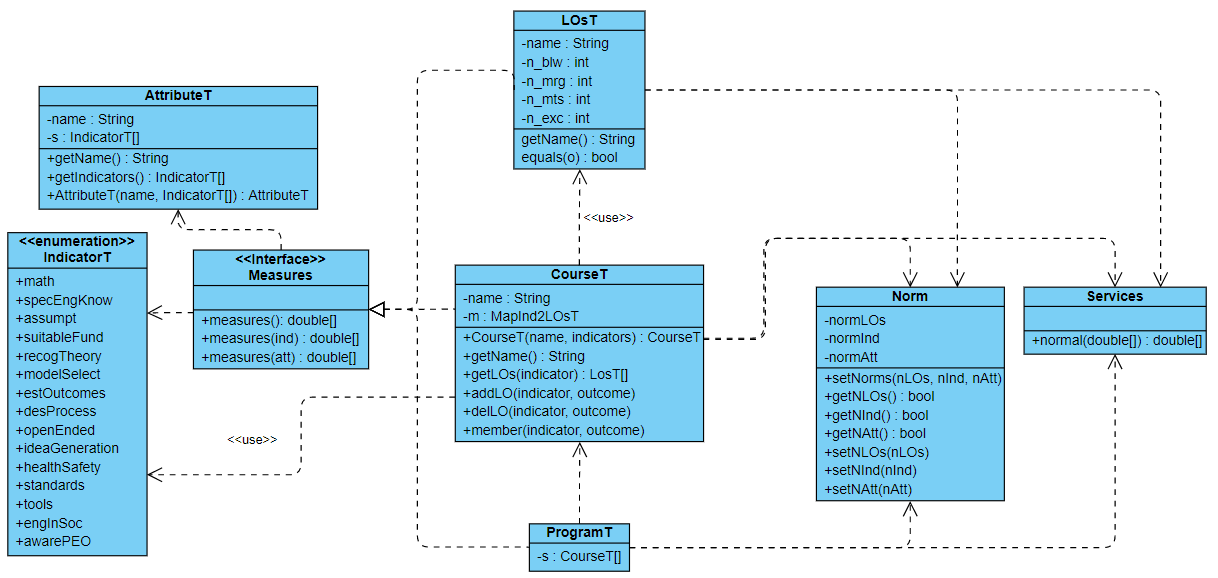
\includegraphics[width=1.0\textwidth]{assets/Q1_UML.png}
	\end{figure}

	\newpage 

	\subsection*{2. Control Flow Graph}
	\begin{figure}[h]
		\centering
		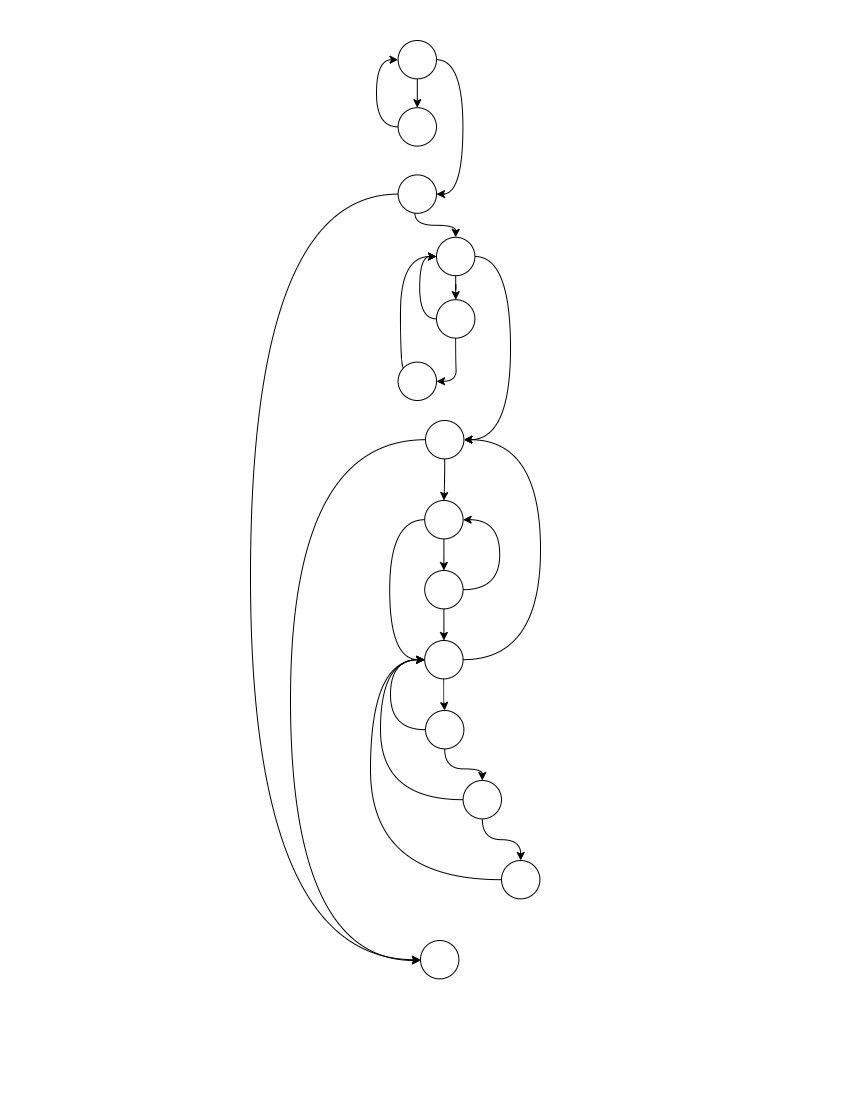
\includegraphics[width=0.75\textwidth]{assets/Q2_ControlFlow.png}
	\end{figure}

\end{document}
